%Correct the file name.
%X: book number
%Y: part number
%ZZZ: page number in three digits. So page 3 would be 003.

\documentclass[11pt]{amsbook}

\usepackage{../HBSuerDemir}	% ------------------------


\begin{document}

% ++++++++++++++++++++++++++++++++++++++
\hPage{b2p1/87}
% ++++++++++++++++++++++++++++++++++++++
\begin{center}
Adj A = $\begin{bmatrix} 
-3 &\ -1 &\ 1 \\
-3 &\  3 &\ 3 \\
3 &\ -1 &\ -5
\end{bmatrix}$ = [$A_{ji}$]
\end{center}

b) Adj B =  $\begin{bmatrix} 
9 &\ -3 \\
-6 &\  2 \\
\end{bmatrix}$

\begin{thm} $A^{-1} $= $\frac{1}{\hAbs{A}}$  Adj A = $\frac{[A_{ji}]}{\hAbs{A}}$ if $\hAbs{A}$ $\neq$ 0, i. e., if $[A_{ij}]$ is invertible.
\end{thm}
\begin{proof} We need to show that

\begin{center}
A $\frac{Adj A}{\hAbs{A}}$ = I or A Adj A = \hAbs{A} I 
\end{center}
Indeed,
\begin{center}
A Adj A = $\begin{bmatrix} 
\cdots &\cdots &\cdots \\
a_{il} &\cdots &\ a_{in} \\
\cdots &\cdots &\cdots
\end{bmatrix}$
$\begin{bmatrix} 
\vdots & A_{lj} &\vdots \\
\vdots &\vdots &\vdots \\
\vdots & A_{nj} &\vdots
\end{bmatrix}$ /$\hAbs{A}$
\end{center}
\begin{center}
\[=[\sum_{\substack{k}} a_{ik} A_{kj}] /\hAbs{A} = [\delta_{ij}\hAbs{A}]/\hAbs{A}= [\delta_{ij}] = I \]
\end{center}
by Theorem 6 on determinant. (Book I)
\end{proof}
\begin{exmp}. Find the inverses of the matrices A and B in Example 1, if any.
\end{exmp}
\begin{hSolution}

a) The classical adjoint of A was obtained as the matrix
\begin{center}
$\begin{bmatrix} 
-3 &\ -3 &\ 3 \\
-1 &\  3 &\  -1 \\
 1 &\  3 &\ -5
\end{bmatrix}$
\end{center}
and the inverse is obtained by dividing this matrix by $\hAbs{A}$= -6
\end{hSolution}
\end{document}  

%==== templates ====

%==== environments ====

%\begin{figure}[htb]
%	\centering
%	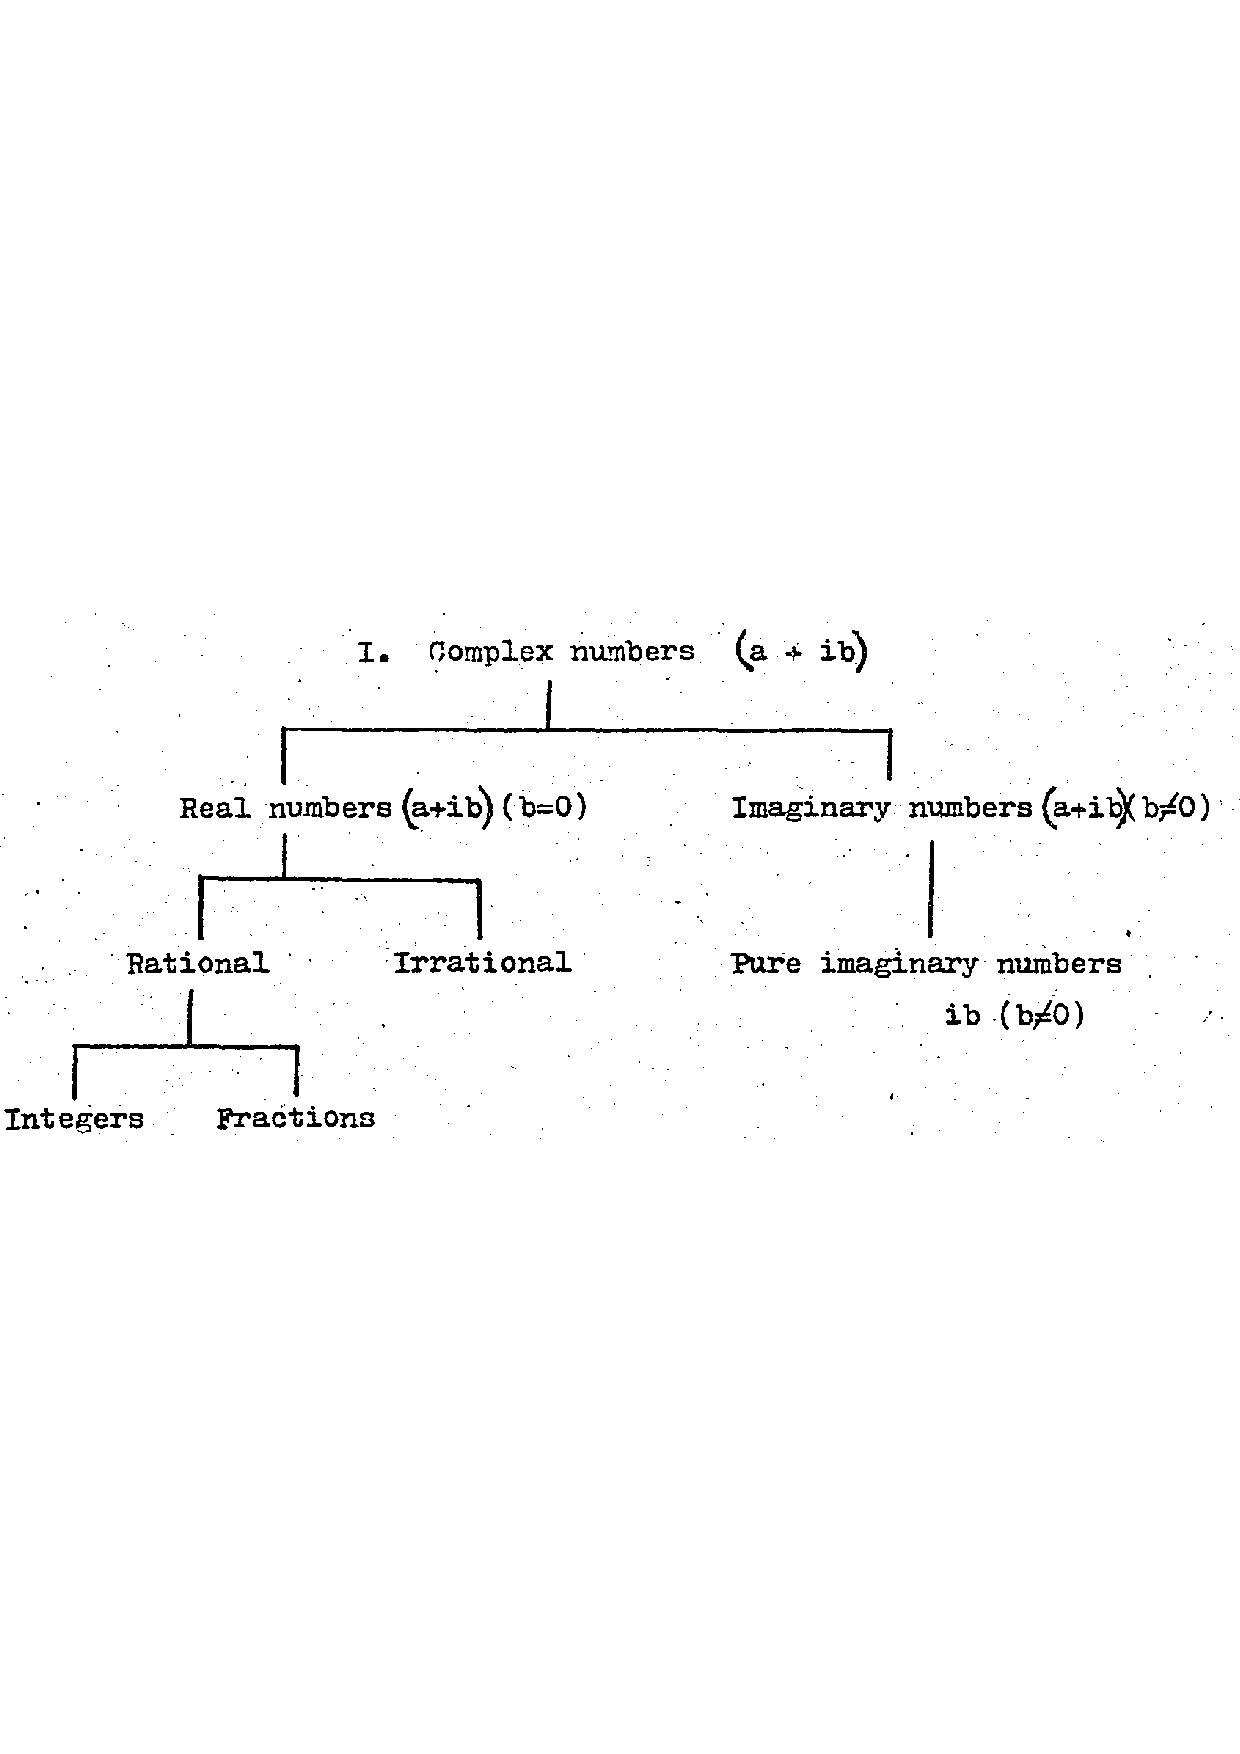
\includegraphics[width=0.9\textwidth]{images/SD-1-1p15A}
%	\caption{Classification of complex numbers}
%	\label{fig:classificationOfComplexNumbersA}
%\end{figure}

%\begin{center}
%\begin{tabular}{cc}
%\end{tabular}
%\end{center}

%\begin{exmp}
%\begin{hSolution}
%\end{hSolution}
%\end{exmp}

%\begin{hEnumerateAlpha}
%\end{hEnumerateAlpha}

%\begin{hEnumerateRoman}
%\end{hEnumerateRoman}

%$
%\begin{bmatrix}
%\end{bmatrix}
%$

%\frac{aaaa}{bbb}
%\frac{a_{n}}{b_{n}}
%\left( aaaa \right)
%\Longrightarrow

%\begin{multicols}{2}
%	bb
%\columnbreak
%	aa
%\end{multicols}
